\documentclass{article}


\usepackage{minitoc}
\usepackage{morefloats}
\usepackage{booktabs}
\usepackage[math]{iwona}
\newsavebox{\savedimage}
\newcommand{\saveimageheight}[2][]{%
  \savebox{\savedimage}{\includegraphics[#1]{#2}}}
\newcommand{\raiseimage}[2][]{%
  \raisebox{.5\dimexpr\ht\savedimage-\height}{%
    \includegraphics[#1]{#2}}}%
%\usepackage{pst-all}
%\usepackage{pst-add}
\usepackage{setspace}
\usepackage{circuitikz}
\usepackage{tikz}
\usepackage{tikz-3dplot}
\usetikzlibrary{decorations.markings,decorations.pathreplacing,calc,patterns,angles,quotes,decorations.pathmorphing,arrows.meta}

\usepackage{multicol}
%\usepackage{lipsum}% dummy text

\setlength{\columnseprule}{0.4pt}

\begin{document}
\centering



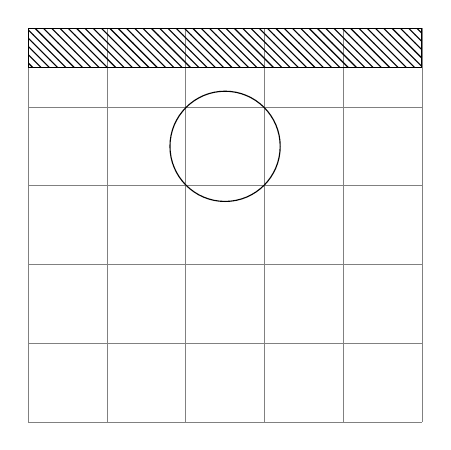
\begin{tikzpicture}

\draw [help lines] (0,0) grid (5,5);

\filldraw [pattern=north west lines] (0,4.5) -- (5,4.5) -- (5,5) -- (0,5) -- cycle;

\draw (2.5, 3.5) circle (0.7);

\end{tikzpicture}

\end{document}
